\documentclass[a4paper,10pt]{article}
\usepackage[utf8]{inputenc}
\usepackage[italian]{babel}
\usepackage{amsmath,amsfonts,amssymb}
\usepackage{graphicx}
\usepackage{float}
\usepackage{siunitx}
\usepackage{geometry}
\geometry{margin=1.5cm}
\usepackage[hidelinks]{hyperref}
\usepackage{array}      % Per migliorare l'allineamento delle celle
\usepackage{booktabs}   % Per linee professionali nella tabella
\usepackage{multicol}
\usepackage{subcaption} % Per i sottotitoli dei subplot
\usepackage{caption}    % Per gestire le didascalie delle figure
\usepackage{circuitikz} % Per disegnare circuiti


\sisetup{per-mode=symbol, detect-all=true}

% Impostazioni per il titolo e l’aspetto generale
\title{\Large\textbf{Terza Esercitazione di Laboratorio}\\ \vspace{0.5em} \large Circuiti RLC in corrente alternata}
\author{\textbf{Gruppo D6/D9:} Cortese Riccardo, Lana Mirko, Saif Edine Safi, Mattia Fait}
\date{\textbf{Novembre 2024}}


\begin{document}
\maketitle
\tableofcontents % Aggiunge un indice interattivo
\newpage

\section*{Materiale Utilizzato e circuito usato per l'esperienza}

Durante l'esecuzione del laboratorio è stato utilizzato il seguente materiale:
\begin{itemize}
    \item breadboard;
    \item cavi bnc, banana-banana e banana-bnc;
    \item resistori \((1k\Omega, 10k\Omega)\);
    \item capacitori \((1nF, 10nF, 100nF)\);
    \item decade di induttanze;
    \item filetti;
    \item generatore di forme d'onda;
    \item oscilloscopio.
\end{itemize}

\begin{figure}[h!]
\centering
\resizebox{0.35\textwidth}{!}{
    \begin{circuitikz}
        % Vin source
        \draw (0,0) to[vsourcesin, l=$V_{\text{in}}(t)$] (0,3) 
            -- (2,3) 
            to[C, l=$C$] (4,3) 
            to[L, l=$L$] (6,3)
            -- (8,3) 
            to[R, l=$R$] (8,0) 
            -- (0,0);
    
        % Ground connection
        \draw (8,0) node[ground] {};
    
        % Vout connection
        \draw (8,3) -- ++(1,0) node[above] {$+$};
        \draw (8,0) -- ++(1,0) node[below] {$-$};
        \node[right] at (9,1.5) {$V_{\text{out}}(t)$};
    \end{circuitikz}
    }
    \caption{Circuito per l'Esercizio 1 e 2}
    
\end{figure}

\section{Diagramma ingresso-uscita (Diagramma di Bode)}

\subsection{Obiettivo}
Con riferimento al circuito di \textit{Figura 1} utilizzando le seguenti combinazioni di R, L, C:
\begin{itemize}
    \item $R = 10 k\Omega, L = 500 mH$ e $C = 10 nF$;
    \item $R = 1 k\Omega, L = 500 mH$ e $C = 10 nF$;
\end{itemize}

si determini il diagramma di Bode del circuito. Si utilizzi una forma d'onda sinusoidale di ampiezza picco-picco $V_{in}^{pp} = 5 V$ con offset pari a zero ($V_{in}^{of} = 0 V$ ). Si utilizzino frequenze da 1 Hz a 50 kHz opportunamente scelte. Si misuri l'ampiezza della forma d'onda in entrata ($V_{in}^{p}$) ed uscita ($V_{out}^{p}$) e la differenza in fase tra le due forme d'onda. 

Si riportino i risultati in due grafici distinti.

Si verifichi se il comportamento del circuito è coerente con le aspettative.

Si stimi la resistenza parassita in serie all'induttore nel caso $R = 1 k\Omega, L = 500 mH$ e $C = 10 nF$.

\subsection{Dati sperimentali}
Di seguito riportiamo due tabelle contenenti le tensioni misurate ad ogni istante di tempo per le diverse combinazioni di R, L e C.

\begin{table}[H]
    \centering
    \begin{minipage}[t]{0.45\textwidth}
        \begin{center}
            \begin{tabular}{|c|c|c|}
                \hline
                Frequenza ($Hz$) & Vout (mV) & Ritardo ($\mu$s)\\
                \hline
                1 & 3.450 & \\
                2 & 6.126 & \\
                5 & 15.250 & \\
                10 & 30.250&\\
                20 & 61 & \\
                50 & 155 & \\
                100 & 301.250 &  \\
                200 & 607.500 &  \\
                500 & 1518 &  \\
                1000 & 2937 & \\
                2000 & 4650 & \\
                2250 & 4775 & \\
                4500 & 3387 & \\
                5000 & 3087 & \\
                10000 & 1506 & \\
                \hline
            \end{tabular}
            \caption{Dati prima combinazione RLC.}
        \end{center}
    \end{minipage}
    \hfill
    \begin{minipage}[t]{0.45\textwidth}
        \begin{center}
           \begin{tabular}{|c|c|c|}
                \hline
                Frequenza ($Hz$) & Vout (mV) & Ritardo ($\mu$s)\\
                \hline
                1 & 0 &\\
                2 & 0 &\\
                5 & 0.675 & \\
                10 & 1.300 & \\
                20 & 2.950 & \\
                50 & 7.875  & \\
                100 & 48.750 & 8079\\
                200 & 61.250 & 6167\\
                500 & 165.375 & 490\\
                1000 & 382.200 & 233\\
                2000 & 2199 & 67\\
                2020 & 2288 & \\
                2250 & 3236 & 1.950\\
                5000 & 397.700 & -254.47\\
                10000 & 159.500 & \\
                \hline
            \end{tabular}
            \caption{Dati seconda combinazione RLC.}
        \end{center}
    \end{minipage}
\end{table}

E' stato scelto di misurare la tensione \textit{$V_{out}$} ad intervalli di frequenza, nel range 1 Hz a 50 Hz, secondo una distribuzione logaritmica.

Oltre a questi dati è stata misurata la tensione \textit{$V_{out}$} nei punti di $f_0$ e $f_{-3db}$ per le due combinazione di R, L e C. 

I dati raccolti si fermano al raggiungimento di frequenza $f = 10 kHz$ in quanto, avendo a disposizione dei cavi lunghi come collegamento tra la decade di induttanze e la breadbord, essi introducevano una induttanza parassita che rendeva l'uscita (Vout) instabile e quindi difficile da misurare.

A puro scopo didattico, abbiamo provato a visualizzare il segnale d'uscita nell'oscilloscopio quando la frequenza $f = 50 kHz$ e abbiamo notato che ad ogni spostamento dei due fili che collegavano la decade di induttanze con la breadbord, il segnale in uscita mutava di volta in volta.

\subsection{Diagrammi di Bode}
Di seguito riportiamo i diagrammi di Bode, ampiezza e fase, relativi alle due combinazioni di R, L e C.

\noindent
I diagrammi sperimentali per l’ampiezza e per la fase si ottengono rispettivamente con le seguenti funzioni:

\begin{minipage} [t]{0.45\textwidth}
    \begin{equation}
        dB = 20log \bigg ( \frac{V_{out}}{V_{in}} \bigg)
    \end{equation}
\end{minipage}
\hfill
 \begin{minipage} [t]{0.45\textwidth}
    \begin{equation}
        \phi[rad] = \frac{\Delta t}{2 \pi \cdot T} 
    \end{equation}
\end{minipage}

 
\begin{figure}[H]
    \centering
    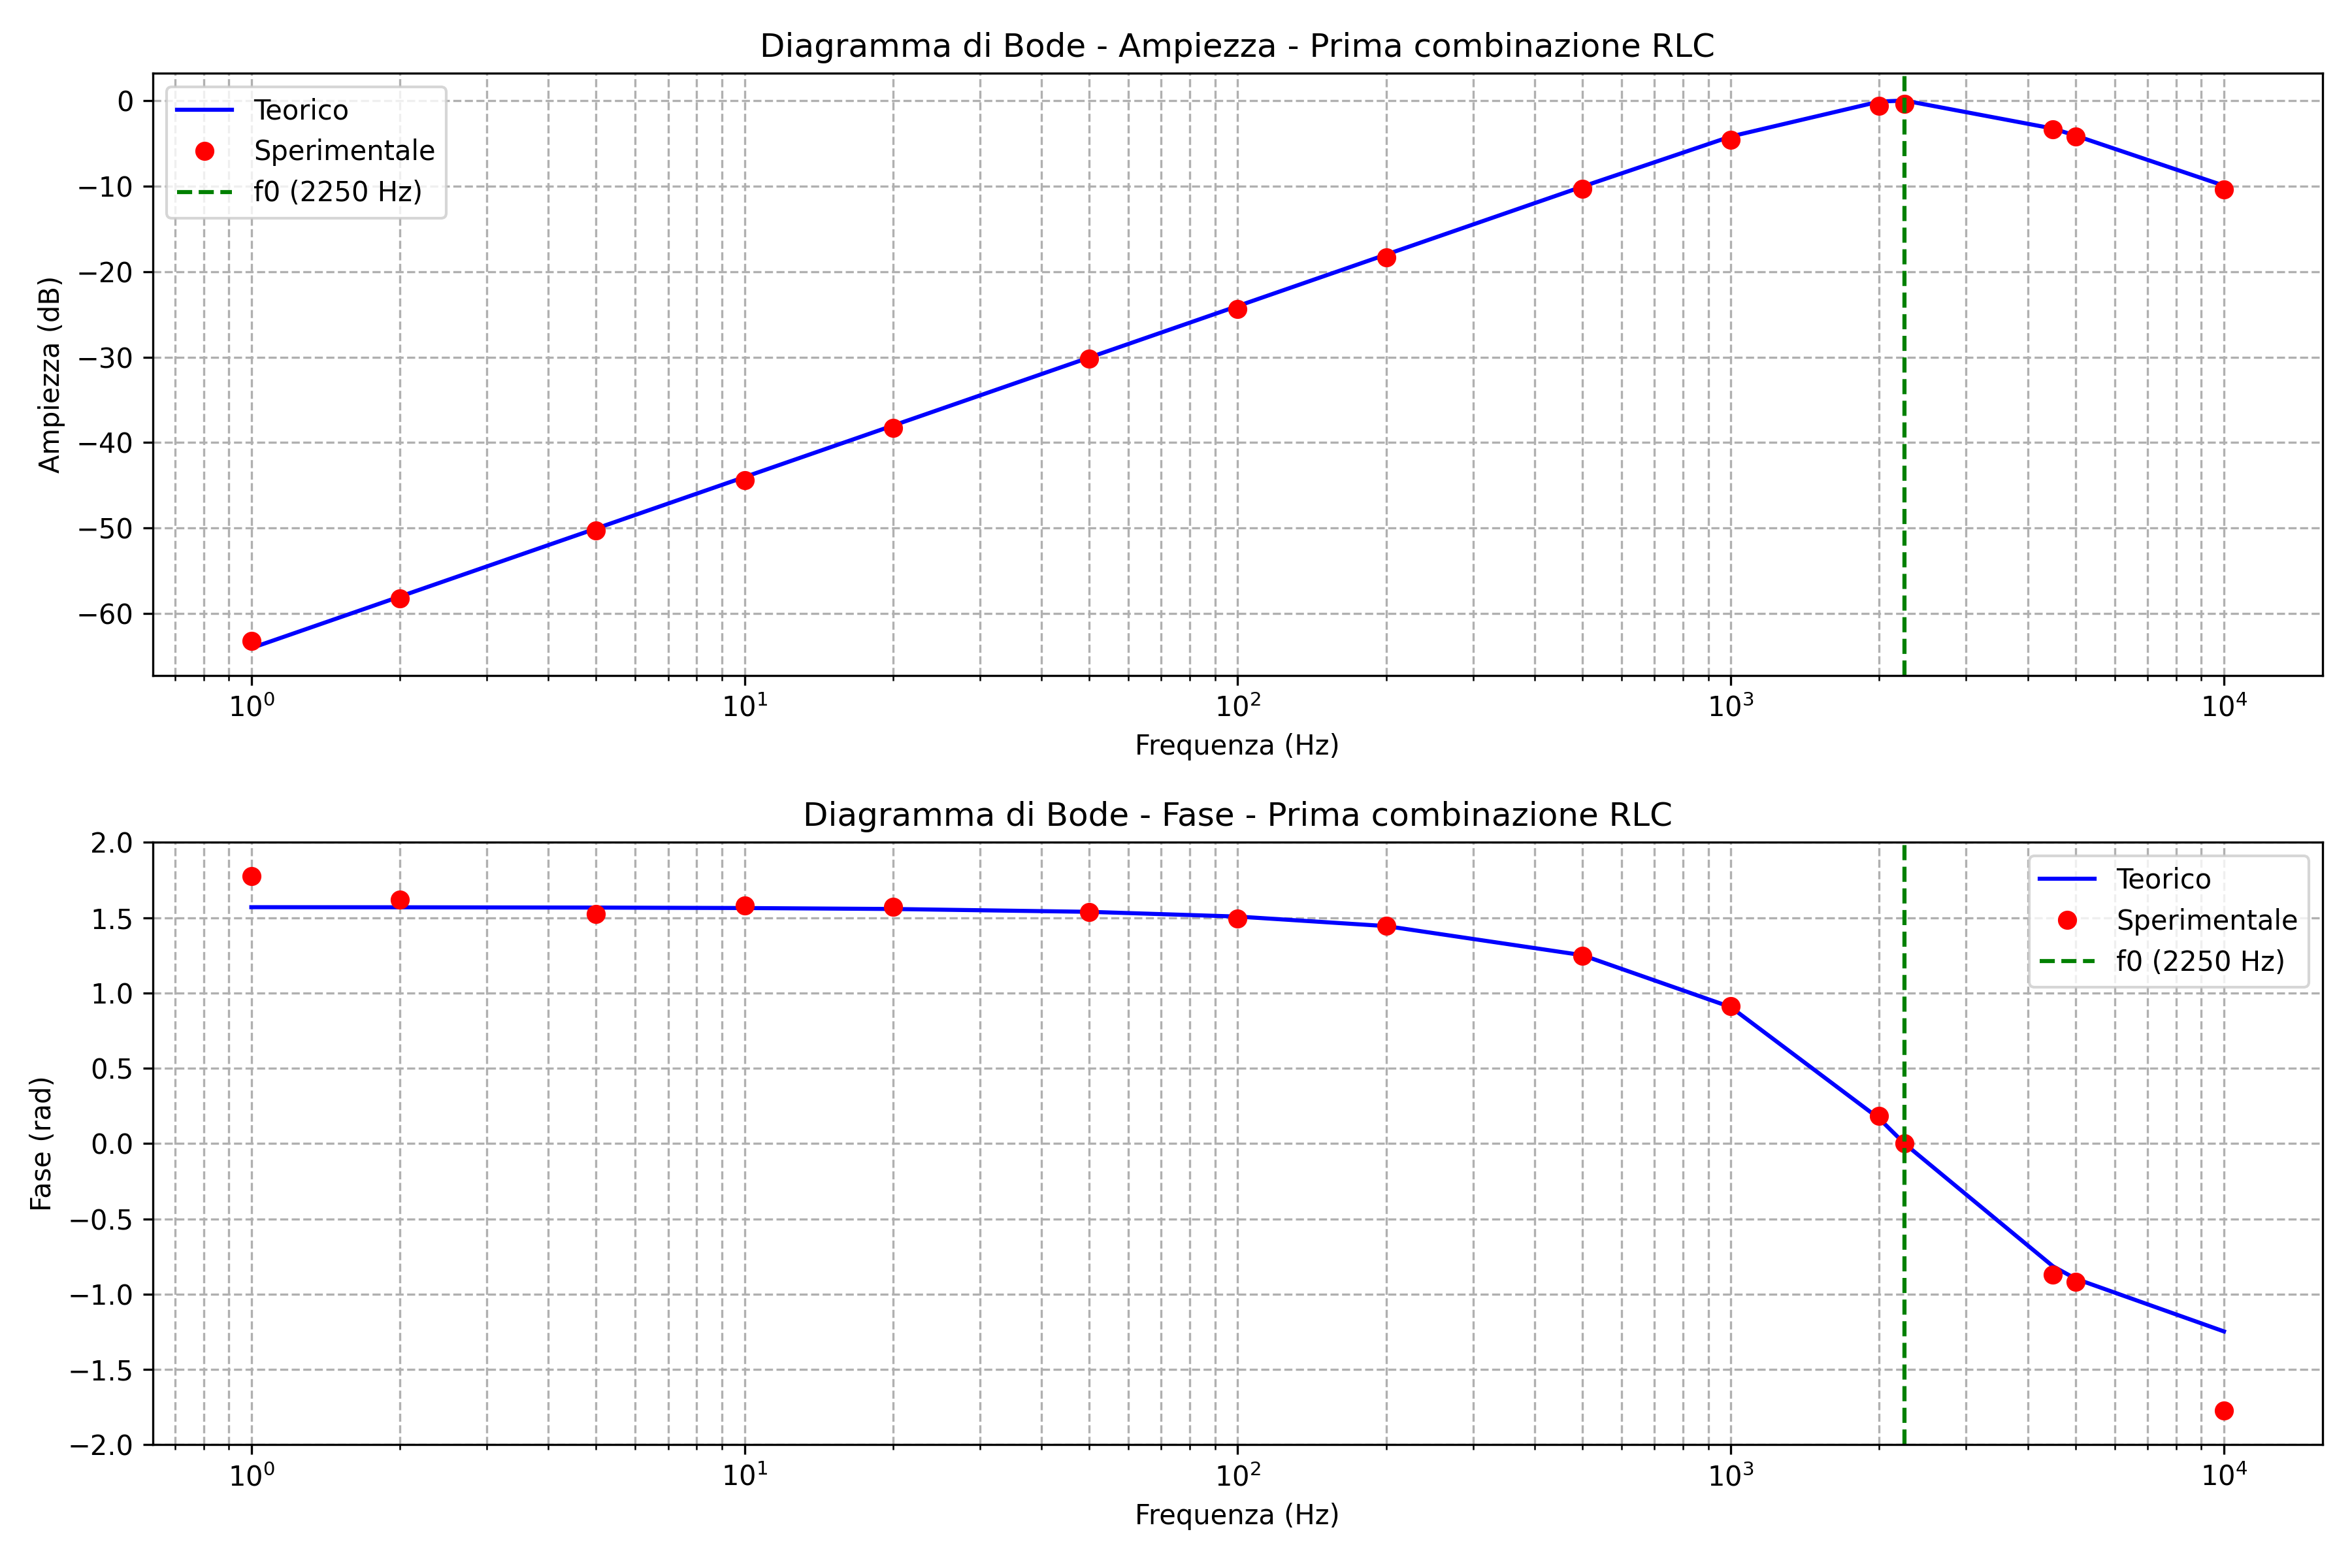
\includegraphics[width=0.7\linewidth]{figures/diagramma_bode_1.png}
\end{figure}
\noindent

\begin{figure}[H]
    \centering
    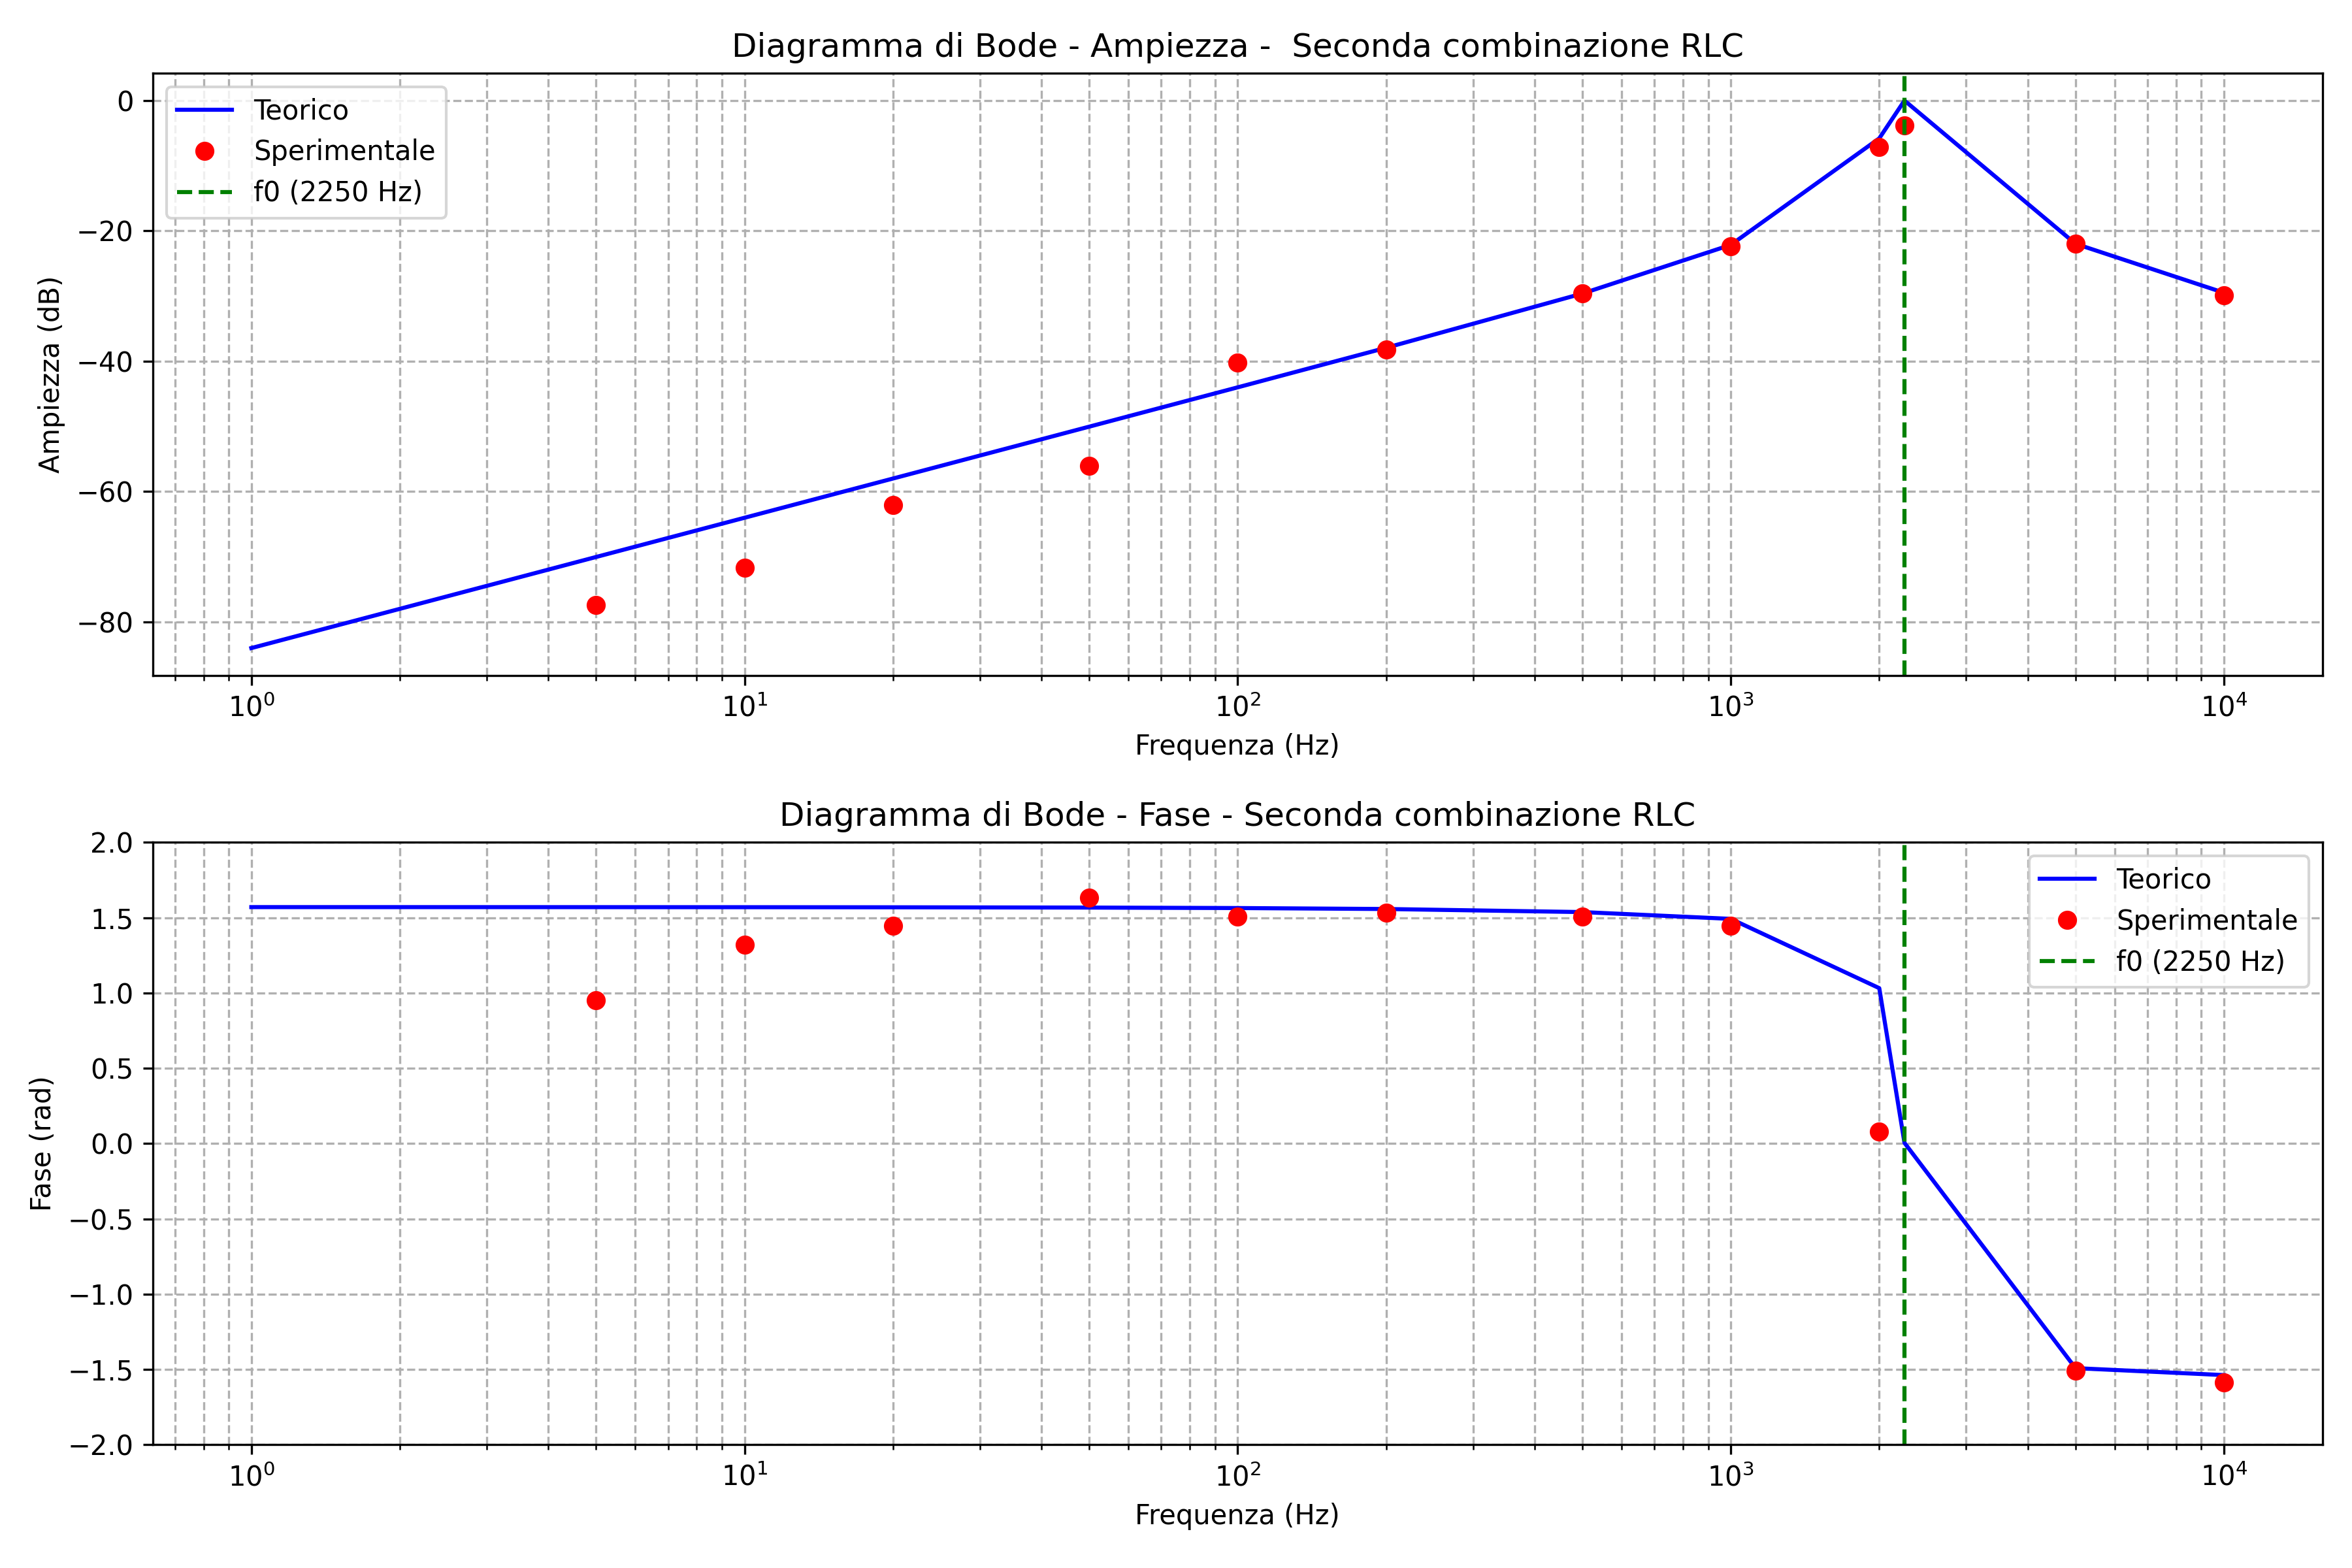
\includegraphics[width=0.7\linewidth]{figures/diagramma_bode_2.png}
\end{figure}
\noindent

I diagrammi sono stati generati tramite codice python da noi implementato.

\subsection{Conclusioni}
Dopo aver calcolato e riportato i diagrammi di Bode per le rispettive combinazioni R, L, e C, possiamo notare come nel primo caso i dati sperimentali rispecchiano l'andamento della curava teorica, a meno di errori sperimentali; nel secondo caso i punti relativi ai dati sperimentali appaiono sottostanti la curva teorica e inoltre a $f_0$ la tensione $V_{out}^{sperimentale} \ll V_{in}$. Questo avviene perchè possiamo immaginare che l'induttore \textit{L} al suo interno abbia una resistenza parassita che determina il calo di tensione. 
Questo avviene perchè l’induttanza è formata da un cavo elettrico attraversato da corrente che si avvolge su se stesso moltissime volte. Più un cavo è lungo più la resistenza parassita è grande

Per trovare questa resistenza parassita possiamo immaginare di avere una resistenza $R_L$ in serie all'induttore $L$ e, per trovare il valore di resistenza di $R_L$, possiamo immaginare di togliere per un momento gli elementi circuitali $C$ e $L$ in modo così di avere un partitore resistivo.

Dalle formule del partitore resistivo: \(V_{out} = \frac{V_{in} \cdot R}{R + R_L}\).

$R_L$ risulterà dunque: \(R_L = \frac{V_{in} \cdot R }{V_{out}} - R \approx 545.117 \Omega \)


\section{Risposta al gradino del circuito RLC}

\begin{multicols}{2}
\subsection{Setup sperimentale}

\begin{itemize}
    \item \textbf{Configurazione circuitale}:
        \begin{itemize}
            \item \textit{circuito RLC in serie} (Figura 1).
        \end{itemize}
    \item \textbf{Segnale in input}:
        \begin{itemize}
            \item \textit{Onda quadra};
            \item Frequenza: \(10 \si{\hertz}\);
            \item Tensione picco-picco: \(2.5 \si{\volt}\);
            \item Offset: \(1.25 \si{\volt}\).
        \end{itemize}
    \item \textbf{Configurazione di test}:
        \begin{itemize}
            \item \(R=10 \si{\kilo \ohm}, L = 500 \si{\milli \henry}, C = 1 \si{\nano \farad}\);
            \item \(R= 10 \si{\kilo \ohm}, L = 500 \si{\milli \henry}, C= 10 \si{\nano \farad}\);
            \item \(R= 10 \si{\kilo \ohm}, L = 100 \si{\milli \henry}, C = 10 \si{\nano \farad}\).
        \end{itemize}
\end{itemize}

\subsection{Obiettivo}

\begin{itemize}
    \item Caratterizzare qualitativamente la \textit{risposta del circuito RLC}:
        \begin{itemize}
            \item Analizzare come il circuito risponde a \textit{differenti valori di L e C};
            \item Focus sulle \textit{frequenze naturali} e \textit{soluzioni del polinomio caratteristico}.
        \end{itemize}
    \item Per la configurazioni \(R = 10 \si{\kilo \ohm}, L = 500 \si{\milli \henry}, C = 1 \si{\nano \farad}\):
        \begin{itemize}
            \item Determinare la \textit{frequenza di oscillazione};
            \item Confrontare il \textit{valore atteso} con quello \textit{osservato}.
        \end{itemize}
\end{itemize}

\end{multicols}


\subsection{Considerazioni}

\begin{itemize}
    \item \textbf{Equazione differenziale del circuito RLC}:
        \begin{itemize}
            \item L'evoluzione del circuito è descritta dall'equazione differenziale
                \begin{equation}
                    L(di/dt)+Ri+(1/C) \int i dt =V_{in}(t)
                \end{equation}
        \end{itemize}
    \item \textbf{Frequenza naturale}:
        \begin{itemize}
            \item La frequenza naturale (\(\omega_n\)) espressa in \(\si{\radian / \second}\) è data da 
                \begin{equation}
                    \omega_n = \frac{1}{\sqrt{LC}}
                \end{equation}
            \item La frequenza naturale (\(f_n\)) espressa in \(\si{\hertz}\) è data da:
                \begin{equation}
                    f_n = \frac{\omega_n}{2 \pi}
                \end{equation}
        \end{itemize}
    \item \textbf{Fattore di smorzamento (Damping Ratio)}:
        \begin{equation}
            \zeta = \frac{R}{2 \sqrt{L/C}}
        \end{equation}
        \begin{itemize}
            \item \(\zeta > 1\) : \textit{Sovrasmorzato} (overdamped);
            \item \(\zeta = 1\) : \textit{Criticamente smorzato};
            \item \(\zeta < 1\) : \textit{Sottosmorzato} (underdamped);
        \end{itemize}
\end{itemize}

\subsection{Analisi del circuito RLC}

\subsubsection{Caso 1}


Per la configurazione \(R=10 \si{\kilo \ohm}, L = 500 \si{\milli \henry}, C = 1 \si{\nano \farad}\) sono stati misurati i seguenti dati:


\begin{table}[h!]
    \centering
        \centering
        \begin{tabular}{|c|c|}
        \hline
        \textbf{Picco di tensione} [\(\si{\milli \volt}\)] & \textbf{Zero misurato} [\(\si{\mu \second}\)] \\
        \hline
        762.5 & 73  \\
        \hline
        355.0 & 146 \\
        \hline
        172.5 & 216 \\
        \hline
        75.0 & 288 \\
        \hline
        12.5 & 361 \\
        \hline
        \end{tabular}
        \caption{Ampiezza misurata in valore assoluto e Zeri di tensione.}
\end{table}
    

\begin{itemize}
    \item \textbf{Frequenza naturale in radianti}
        \[\omega_n = \frac{1}{\sqrt{(500 \si{\milli \henry})\cdot(1 \si{\nano \farad})})} \approx 44721 \si{\radian / \second}\]

    \item \textbf{Frequenza naturale in hertz}
        \[f_n = \frac{\omega_n}{2 \pi} \approx 7118 \si{\hertz}\]

    \item \textbf{Frequenza di oscillazione} \\
        La frequenza di oscillazione sperimentale \(f_o=\frac{\omega_o}{2 \pi}\) si può ricavare dal periodo di oscillazione \(T_o\) della curva in uscita, infatti \(f_o = \frac{1}{T_o}\).   \\
        Il periodo di oscillazione è il tempo che impiega la curva per effettuare un'oscillazione completa.
        
        \[T_o = 72 \si{\mu \second} \cdot 2 = 144 \si{\mu \second} \Rightarrow f_o = \frac{1}{144 \si{\mu \second}} \approx 6944 \si{\hertz}\]

        Il risultato sperimentale è in accordo con il risultato teorico, pur essendoci un errore pari a \(f_n -f_o \approx 174 \si{\hertz}\), dovuto probabilmente alla sensibilità della strumentazione di laboratorio.
    
    \item \textbf{Fattore di smorzamento}
        \[\zeta = \frac{10 \si{\kilo \ohm}}{2 \cdot \sqrt{(500 \si{\milli \henry})/(1 \si{\nano \farad})}} \approx 0.224\]
        Poiché \(\zeta <1\), il circuito è sottosmorzato e la risposta sarà oscillante e la soluzione sarà caratterizzata da una smorzatura epsonenziale descritta da
        \[L \frac{d^2 e^{\lambda t}}{dt}+R \frac{d e^{\lambda t}}{dt} + \frac{2^{\lambda t}}{C} =0\]
        \(\forall \, \lambda = -\zeta \omega_0 \pm j \omega_0 \sqrt{1- \zeta^2}\). \\
        La risposta al gradino avrà quindi oscillazioni che decresceranno nel tempo, come è stato provato dalle misure sperimentali mostrate in Figura 2.

        \begin{figure}[h!]
            \centering
            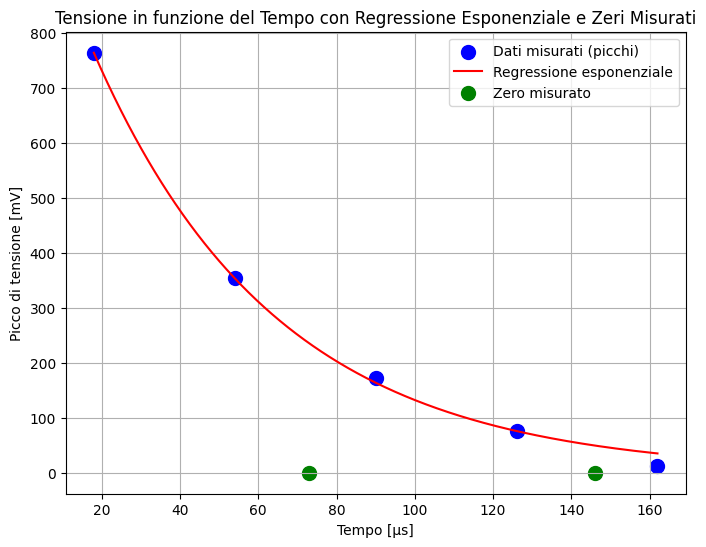
\includegraphics[width=0.4\textwidth]{figures/regr_exp.png}
            \caption{Oscillazioni sperimentali decrescenti nel tempo.}
        \end{figure}

\end{itemize}


%\newpage

\subsubsection{Caso 2}

\(R= 10 \si{\kilo \ohm}, L = 500 \si{\milli \henry}, C= 10 \si{\nano \farad}\);


\begin{itemize}
    \item \textbf{Frequenza naturale in radianti}
        \[\omega_n = \frac{1}{\sqrt{(500 \si{\milli \henry})\cdot(10 \si{\nano \farad})})} \approx 14142 \si{\radian \second}\]

    \item \textbf{Frequenza naturale in hertz}
        \[f_n = \frac{\omega_n}{2 \pi} \approx 2251 \si{\hertz}\]
    \item \textbf{Fattore di smorzamento}
        \[\zeta = \frac{10 \si{\kilo \ohm}}{2 \cdot \sqrt{(500 \si{\milli \henry})/(10 \si{\nano \farad})}} \approx 0.707\]
        Circuito sottosmorzato.
        \[L \frac{d^2 e^{\lambda t}}{dt}+R \frac{d e^{\lambda t}}{dt} + \frac{2^{\lambda t}}{C} =0\]
        \(\forall \, \lambda = -\zeta \omega_0 \pm j \omega_0 \sqrt{1- \zeta^2} \). \\
        La risposta mostrerà oscillazioni, ma il loro smorzamento sarà più rapido rispetto al caso precedente, grazie ad un fattore di smorzamento più alto. \\
        La risposta si stabilizzerà più velocemente.
\end{itemize}




\subsubsection{Caso 3}

\(R= 10 \si{\kilo \ohm}, L = 100 \si{\milli \henry}, C = 10 \si{\nano \farad}\).


\begin{itemize}
    \item \textbf{Frequenza naturale in radianti}
        \[\omega_n = \frac{1}{\sqrt{(100 \si{\milli \henry})\cdot(1 \si{\nano \farad})})} \approx 31623 \si{\radian \second}\]
    \item \textbf{Frequenza naturale in hertz}
        \[f_n = \frac{\omega_n}{2 \pi} \approx 5033 \si{\hertz}\]
    \item \textbf{Fattore di smorzamento}
        \[\zeta = \frac{10 \si{\kilo \ohm}}{2 \cdot \sqrt{(100 \si{\milli \henry})/(1 \si{\nano \farad})}} \approx 1.58\]
        Poiché il circuito è sovrasmorzto (\(\zeta > 1\)), la risposta non oscillerà ma crescerà lentamente verso il valore finale e la soluzione caratteristica sarà caratterizzata da una smorzatura esponenziale descritta da 
        \[L \frac{d^2 e^{\lambda t}}{dt}+R \frac{d e^{\lambda t}}{dt} + \frac{2^{\lambda t}}{C} =0\]
        \(\forall \, \lambda = \frac{-R \pm \sqrt{R^2 -4L \cdot \frac{1}{C}}}{2L}\).\\
        La risposta a un ingresso a gradino vedrà un'espansione iniziale senza oscillazioni, ma ci vorrà più tempo per raggiungere il valore finale.

\end{itemize}




\end{document}
